
\chapter{Examples and applications}
Most of this chapter is optional; sometimes the first two sections will be useful in later chapters, but the later sections will only be used in motivational sections, exercises, and examples.
The point here is to bring the level of abstraction down and show what one can do with all the machinery that we built up last chapter.

\section{Measurable maps}
In topology, a continuous map is one that pulls back open sets to open sets.
Here we have no open sets to work with --- only measurable sets --- but this turns out to be exactly what we want.

\begin{definition}
Let $(X, \Sigma)$ and $(Y, \Gamma)$ be measurable spaces.
A \dfn{measurable map} $f: X \to Y$ is a map such that for every measurable set $A \in \Gamma$, $f^{-1}(A)$ is measurable.

A \dfn{measurable isomorphism} is a measurable map $f: X \to Y$ such that $f$ is a bijection and $f^{-1}$ is measurable.
If a measurable isomorphism exists, we say that $X,Y$ are \dfn{isomorphic} as measurable spaces, or that $\Sigma$ and $\Gamma$ are \dfn{isomorphic} as $\sigma$-algebras.
\end{definition}

\begin{example}
Isomorphism of measurable spaces is a very weak notion.
If $X$ is an uncountable \dfn{Polish space} --- a complete separate metric space --- then we call its Borel $\sigma$-algebra $\Sigma$ the \dfn{standard Borel algebra}.
A theorem of a branch of logic known as descriptive set theory implies that there is only one standard Borel algebra, up to isomorphism.
So any two Polish spaces, when viewed as measurable spaces, are the same!
\end{example}

\begin{definition}
Let $(X, \Sigma, \mu)$ be a measured space, $(Y, \Gamma)$ a measurable space, and $f: X \to Y$ a measurable map.
We define $f_{*}(\mu)$ on $(Y, \Gamma)$ by
\[f_{*}(\mu)(E) = \mu(f^{-1}(E))\]
and call $f_{*}(\mu)$ the \dfn{pushforward measure} of $\mu$ by $f$.
\end{definition}

\begin{example}\label{lebesgue measure torus}
Let $\Torus$ be the circle, viewed for now as the set $\{z \in \CC: |z| = 1\}$.
Then $\Torus$ has its Borel $\sigma$-algebra $\Gamma$.
Let $\Sigma$ be the Borel $\Sigma$-algebra of $\RR$ and $\mu$ the Lebesgue measure restricted to $\Sigma$.
Then we have a continuous map $f: [0, 1] \to \Torus$ defined by
\[f(x) = e^{2\pi ix}.\]
Every continuous map between Borel measurable spaces is measurable, so $f$ is.
The pushforward measure $\nu = f_{*}(\mu)$ is known as the \dfn{Lebesgue measure} on $\Torus$.
The diligent reader will check that $\nu$ agrees with the notion of arc length defined in multivariable calculus (Exercise~\ref{arc length exercise}).
\end{example}

\begin{definition}
Let $(X, \mu)$ and $(Y, \nu)$ be measured spaces.
A \dfn{measure-preserving map} is a measurable map $f: X \to Y$ such that
\[\nu = f_{*}(\mu).\]
If $f$ is a measurable isomorphism, we call $f$ a \dfn{measure-preserving isomorphism}.
\end{definition}

\begin{definition}
Let $X$ be a set, $(Y, \Gamma)$ a measurable space, and $F: X \to Y$ a map.
The \dfn{pullback $\sigma$-algebra} $F^{*}\Gamma$ is the $\sigma$-algebra of sets of the form $F^{-1}(A)$ where $A \in \Gamma$.
\end{definition}

\begin{subsec}
We need to check that the definition of a pullback $\sigma$-algebra makes sense.
Namely, we must show that if $F: X \to Y$ is a map, and $\Gamma$ a $\sigma$-algebra on $Y$, then $F^{*}\Gamma$ is a $\sigma$-algebra.
This is part of the content of Exercise~\ref{pullback makes sense}, which also shows that $F^{*}\Gamma$ is the smallest $\sigma$-algebra for which $F$ is measurable.
\end{subsec}

\begin{exercise}
Show that measurable spaces with measurable maps form a category.
\end{exercise}

\begin{exercise}\label{arc length exercise}
By an \dfn{arc} we mean a compact connected subset of $\Torus$.
Recall the definition of the length of an arc from calculus.
Show that the length of an arc equals its Lebesgue measure.
\end{exercise}

%\begin{exercise}\label{Lebesgue measure on sphere}
%Let $S^{d}$ denote the unit sphere in $\RR^{d+1}$, and let $N$ be its open northern hemisphere.
%Let $U$ be the open unit ball in $\RR^{d}$, so $U \times \{0\}$ is a subset of the unit ball of $\RR^{d+1}$.
%Show that the map $p: N \to \RR^{d+1}$, $p(x_{1}, \dots, x_{d+1}) = (x_{1}, \dots, x_{d}, 0)$, is a homeomorphism between $N$ and $U \times \{0\}$.
%So the pushforward of Lebesgue measure on $\RR^{d}$ by $p^{-1}$ gives a Borel measure on $N$, which we call \dfn{Lebesgue measure} on $N$.
%Use this fact to define Lebesgue measure of any Borel subset of $S^{d}$.
%Show that when $d = 2$, Lebesgue measure on $S^{d}$ agrees with the usual notion of surface area, up to a constant factor.
%\end{exercise}
% I think this exercise is just wrong !

\begin{exercise}\label{pullback makes sense}
Let $F: X \to Y$ be a map, $\Gamma$ a $\sigma$-algebra on $Y$.
Show that $F^{*}\Gamma$ is a $\sigma$-algebra on $X$ and $F: (X, F^{*}\Gamma) \to (Y, \Gamma)$ is measurable.
Conversely, show that $F^{*}\Gamma$ is the intersection of all $\sigma$-algebras $\Sigma$ on $X$ such that $F: (X, \Sigma) \to (Y, \Gamma)$ is measurable.
\end{exercise}

\section{Probability}
In 1933, Andrey Kolmogorov put probability theory --- which was long viewed as not part of rigorous mathematics --- on a sound footing by establishing three axioms that probability theory ought to satisfy.
These axioms, however, are exactly the definition of a probability measure!
Thus measure theory is an invaluable tool in applied mathematics, such as statistics.
However, even the myopic reader who only cares about pure, abstract mathematics will find probability useful to their work.

In this section we do little more than develop a language, but in later sections we will find a great use for it.

\begin{definition}
A \dfn{probability space} $(\Omega, \Sigma, P)$ is a measure space with $P(\Omega) = 1$.
Elements of $\Sigma$ are called \dfn{events} and elements of $X$ are called \dfn{outcomes}.
The quantity $P(A)$, where $A$ is an event, is called the \dfn{probability} that $A$ is true.
\end{definition}

\begin{subsec}
The intuition here is that the events form an algebra $\Sigma$ of statements that could be true or false about the world, with varying probabilities.
By an algebra of statements, more precisely, one means that it is meaningful to conjoin them using grammar: $A \cup B$ is the event that $A$ happens or $B$ happens, while $A \cap B$ is the probability that both $A$ happens and $B$ happens. The event $\Omega \setminus A$ is the probability that $A$ does not happen, and so on.
The event $\Omega$ is vacuously true; it represents the statement ``$2 + 2 = 4$''.
The event $\emptyset$, on the other hand, is vacuously false; it represents the statement ``$2 + 2 = 5$''.
Thus probability theory sits somewhere between analysis and logic in the world of mathematics, and the language used in the following definition is motivated.
\end{subsec}

\begin{definition}
Let $(\Omega, \Sigma, P)$ be a probability space.

The event $A \cup B$ is called $A$ \dfn{or} $B$, or the \dfn{disjunction} of $A,B$, and the event $A \cap B$ is called $A$ \dfn{and} $B$, or the \dfn{conjunction} of $A,B$.
The event $\Omega \setminus A$ is called \dfn{not} $A$, or the \dfn{negation} of $A$.

The event $\Omega$ is said to be \dfn{true}, and the negation $\emptyset$ of true is said to be \dfn{false}.
An event $A$ is said to be \dfn{almost surely true} if $P(A) = 1$, and \dfn{almost surely false} if $P(A) = 0$.

A set $\Sigma_{0} \subseteq \Sigma$ of events is said to be \dfn{mutually exclusive} if for every $A, B \in \Sigma_{0}$, $A \cap B$ is almost surely false.
\end{definition}

\begin{subsec}
The $\sigma$-additivity of the measure $P$ says that if a countable set $\Sigma_{0}$ of events is mutually exclusive, its disjunction $A$ satisfies
\[P(A) = \sum_{B \in \Sigma_{0}} P(B),\]
thus for example we have the \dfn{inclusion-exclusion formula}
\[P(E \cup F) = P(E) + P(F) - P(E \cup F)\]
valid for any two events $E,F$ familiar from elementary probability theory.
\end{subsec}

\begin{subsec}
So far we have only discussed events. But what role do outcomes play?
Outcomes are ``microstates'' and each outcome carries all possible information about a particular state that the universe could be --- the position and momentum of every last molecule, the value of every card in every player's hand.
But we are just puny mortal observers of the universe; we cannot possibly have access to all that information!
So outcomes are not terribly useful, and one generally avoids ever mentioning outcomes directly.
What we mortal observers can observe are random variables.
\end{subsec}

\begin{definition}
Let $(\Omega, P)$ be a probability space and $E$ be a measurable space.
A \dfn{random variable} of \dfn{type} $E$, also known as an \dfn{observable} of type $E$, is a measurable map $\Omega \to E$.
\end{definition}

\begin{subsec}
The points of the space $E$ represent possible values that an experiment can return.
The random variable $X: \Omega \to E$ represents an experiment. If $\omega$ is an outcome, $X(\omega)$ is the result of the experiment $X$ if the universe is in state $\omega$.
One generally takes $E = \RR$ with its Borel $\sigma$-algebra, since most experiments return numerical data, but there are other examples of useful types $E$; for example, points of $E$ are often sequences, vectors, or graphs.
If the type of $X$ is clear --- especially if it is $\RR$ --- we will suppress it.
\end{subsec}

\begin{subsec}
Let $X$ be a random variable (of type $\RR$).
The sets $[x, \infty)$ are Borel, so the sets $\{X \geq x\} = \{\omega \in \Omega: X(\omega) \geq x\}$ are actually events.
The probability of the event $\{X \geq x\}$ is frequently of interest, so we make the following definition.
\end{subsec}

\begin{definition}
Let $X$ be a random variable of type $E$.
The \dfn{distribution} $\mu_{X}$ of $X$ is the pushforward $X_{*}P$ of $P$ on $E$.
If $Y$ is another random variable and $\mu_{X} = \mu_{Y}$, we say that $X,Y$ are \dfn{identically distributed}.
\end{definition}

\begin{subsec}
Unraveling the definitions, if $A \subseteq E$ is a measurable set,
\[\mu_{X}(A) = P(X \in A) = P(\{\omega \in \Omega: X(\omega) \in A\}).\]
For example, if $E = \RR$ then $\mu_{X}([x, \infty))$ is the probability that $X \geq x$.
We think of two identically distributed random variables as being isomorphic, but not the same.
\end{subsec}

\begin{figure}\label{bell curve figure}
\caption{A Gaussian cdf (in blue) and its derivative, the familiar ``bell curve'' from elementary statistics (in green).}
\centering 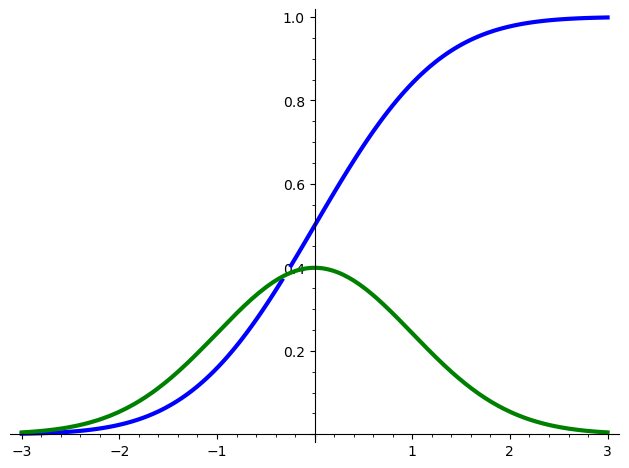
\includegraphics[width=0.5\textwidth]{graphics/bell_curve}
\end{figure}

\begin{example}\label{Gaussian CDF}
An especially important and familiar distribution is the \dfn{Gaussian measure} $N(0, 1)$ on $\RR$, which is the Stieltjes measure defined by the \dfn{Gaussian cumulative distribution function} (or \dfn{Gaussian cdf})
\[f(x) = \frac{1}{\sqrt{2\pi}} \int_{-\infty}^{x} \exp\left(-\frac{y^{2}}{2}\right) ~dy.\]
In other words, the measure of $[\alpha, \beta)$ is by definition $f(\beta) - f(\alpha)$.
Here the factor of $1/\sqrt{2\pi}$ is to ensure that $N(0, 1)$ is actually a probability measure, c.f. Example~\ref{Gaussian integral formula}.
A random variable with distribution $N(0, 1)$ is said to be a \dfn{standard-normally distributed} random variable. More generally, one defines $N(\mu, \sigma^{2})$ to be the Stieltjes measure defined by the cumulative distribution function
\[x \mapsto \frac{1}{\sigma\sqrt{2\pi}} \int_{-\infty}^{x} \exp\left(-\frac{1}{2}{\left(\frac{y - \mu}{\sigma}\right)}^{2}\right) ~dy,\]
and a random variable with distribution $N(\mu, \sigma^{2})$ is said to be \dfn{normally distributed} with mean $\mu$ and standard deviation $\sigma$.
See Figure~\ref{bell curve figure}.
\end{example}

\begin{subsec}
Recall that in elementary probability theory two events $A,B$ are said to be independent if $P(A) = P(A|B)$, where $P(A|B)$ (``the probability of $A$ given $B$'') is by definition $P(A \cap B)/P(B)$.
The intuition is that if we know that $B$ is true, then we want to restrict to subsets of $B$ and rescale the probability measure $P$ so that $B$ is almost surely true.
However, if $A$ and $B$ really have nothing to do with each other, the probability of $A$ given $B$ is just the probability of $A$.
We can write this in a more symmetrical form, which also avoids the issue of division by zero, as in the following definition.
\end{subsec}

\begin{definition}
Let $(\Omega, \Sigma, P)$ be a probability space and $(E, \Gamma)$ a measurable space.

Countably many events $A_{n} \in \Sigma$ are said to be \dfn{independent} if
\[P\left(\bigcap_{n} A_{n}\right) = \prod_{n} P(A_{n}).\]
Countably many $\sigma$-algebras $\mathcal A_{n} \subseteq \Sigma$ are said to be \dfn{independent} if for every $A_{n} \in \mathcal A_{n}$, the events $A_{n}$ are independent.
Countably many random variables $X_{n}$ of type $E$ are said to be \dfn{independent} if the pullback $\sigma$-algebras $X_{n}^{*}\Gamma$ are independent.

Random variables $X,Y$ are said to be \dfn{iid} if they are independent and identically distributed.
\end{definition}

\begin{subsec}
The idea in the definition of independent random variables is that the pullback $\sigma$-algebra $X^{*}\Gamma$ is the set of events that can be checked as true or false by measuring $X$.
\end{subsec}

\begin{example}
Suppose that I am playing a game of cards.
Every time I draw a card, I put it back in the deck and then shuffle again.
Let $X_{n}$ be $1$ if I draw the queen of hearts on turn $n$, and $0$ otherwise.
Then the distribution of $X_{n}$ is $(51/52)\delta_{0} + (1/52)\delta_{1}$, where $\delta_{x}$ is the Dirac measure at $x$.
Since I shuffle between turns, the $X_{n}$ are independent.
So the $X_{n}$ are iid.
\end{example}

\begin{exercise}
Verify the inclusion-exclusion formula
\[P\left(\bigcup_{i=1}^{n} A_{i}\right) = \sum_{k=1}^{n} {(-1)}^{k+1} \sum{1 \leq i_{1} < \cdots < i_{k} \leq n} P\left(\bigcap_{j=1}^{k} A_{i_{j}}\right)\]
valid for any events $A_{1}, \dots, A_{n}$.
\end{exercise}

\begin{exercise}[Skohorod representation]\label{Skohorod representation}
Let $\mu$ be a Borel probability measure on $\RR$.
Show that there is a probability space $\Omega$ and a random variable $X: \Omega \to \RR$ of distribution $\mu$.
\end{exercise}

\begin{exercise}
Let $X_{n}$ be random variables and suppose that for every $x \in \RR$, the events $X_{n} \geq x$ are independent.
Show that the $X_{n}$ are independent random variables.
\end{exercise}

\begin{exercise}
Let $X_{n}$ be independent random variables of type $E$.
Suppose that $f_{n}: E \to E$ are measurable maps.
Show that the $f_{n}(X_{n})$ are still independent.
\end{exercise}

\begin{exercise}
Let $X, Y: \Omega \to E$ be random variables.
A \dfn{morphism of random variables} $X \to Y$ is a measure-preserving map $F: \Omega \to \Omega$ such that $Y \circ F = X$.
Two morphisms $F,G$ are \dfn{equal almost surely} if $P(F = G) = 1$.
Two random variables $X,Y$ are \dfn{isomorphic} if there are morphisms $F: X \to Y$ and $G: Y \to X$ such that $F \circ G$ and $G \circ F$ are the identity almost surely (so $G$ is almost surely the inverse of $F$).

Show that being equal almost surely is an equivalence relation on the set of morphisms of random variables.
Show that random variables $\Omega \to E$ and morphisms between them, modulo the equivalence relation of being equal almost surely, form a category.
Show that two random variables are isomorphic iff they are identically distributed.
\end{exercise}



\section{Hausdorff measures}
At this point we have defined Stieltjes measures.
In particular, we defined the Lebesgue measure and the Dirac measure.
Let us treat some more measures. This section is optional, as it is only used in some examples; one could, at least in principle, take the spherical Lebesgue measure as a black box.

Our first motivation for this section comes from the Cantor set $C$.
In some ways, $C$ is quite large, since it is uncountable. But Lebesgue measure does not recognize this; it only recognizes that $C$ is a null set, and so according to Lebesgue measure, $C$ is no larger than the empty set!

But Lebesgue measure is hardly the only measure guilty of this. The area of a circle, or the volume of a plane, are both zero -- but when we pass to a lower-dimensional measure, namely the arc length of a circle, or the area of a plane, suddenly we can tell the difference between them and the empty set.
This suggests that the problem with the Cantor set is that it is in some sense lower-dimensional than the line, which is one-dimensional.

\begin{subsec}
Recall that Lebesgue measure $\mu$ is outer regular, so it satisfies, for every Borel set $E$,
$$\mu(E) = \inf\left\{\sum_{n=1}^\infty \mu(U_n): \mu(U_{n})~\text{open},~E \subseteq \bigcup_{n=1}^\infty U_{n}\right\}.$$
Since every open subset of $\RR$ can be written as a countable union of open intervals $(\alpha, \beta)$, and the Lebesgue measure of an open interval $(\alpha, \beta)$ satisfies $\mu((\alpha, \beta)) = \beta - \alpha = \sup_{\alpha < x,y < \beta} |x - y|$, this is nothing more than
\begin{equation}
\label{motivating Hausdorff}
\mu(E) = \inf\left\{\sum_{n=1}^\infty \diam U_{n}: U_{n}~\text{open},~E \subseteq \bigcup_{n=1}^\infty U_{n}\right\}
\end{equation}
where the \dfn{diameter} of an open set $U$ is defined by $\diam U = \sup_{x,y \in U} |x - y|$.

Now, recall some high school geometry: the volume of a $d$-dimensional ball $U$ is proportional to $(\diam U)^{d}$.
This suggests that if we want to know the $d$-dimensional measure of a set, we need to replace $\diam U_{n}$ with $(\diam U_{n})^{d}$ in (\ref{motivating Hausdorff}).
\end{subsec}

\begin{definition}
The \dfn{$d$-dimensional Hausdorff outer measure} is defined on sets $E \subseteq \RR^k$ by
$$\mathcal H^d(E) = \inf\left\{\sum_{n=1}^\infty (\diam U_{n})^d: U_{n}~\text{open},~E \subseteq \bigcup_{n=1}^\infty U_{n}\right\}.$$
The \dfn{$d$-dimensional Hausdorff measure}, also denoted $\mathcal H^d$, is the restriction of $\mathcal H^d$ to $\mathcal H^d$-measurable sets.
\end{definition}

\begin{subsec}
We now check that Hausdorff measure is well-defined.
First, according to Exercise~\ref{Hausdorff is outer measure}, $\mathcal H^d$ is an outer measure.
Thus, by Carathéodory's theorem, the $\mathcal H^d$-measurable sets -- that is, those sets which cleanly divide every subset of $\RR^k$ with respect to $\mathcal H^d$ -- form a $\sigma$-algebra $\Sigma$ and $\mathcal H^d|\Sigma$ is honestly a measure.
However, this is not a priori very useful.
After all, $\Sigma$ could be the trivial $\sigma$-algebra!
We will need to show that $\Sigma$ contains the Borel sets in order for $\mathcal H^d$ to be useful.
In order to do so, we will need some general facts about outer measures on metric spaces.
If the reader is uncomfortable with metric spaces, they can take $X = \RR^d$ and $d(x, y) = |x - y|$ and not miss out on any of the key ideas here.
\end{subsec}

\begin{definition}
Let $(X, d)$ be a metric space.
If $A, B$ are nonempty subsets of $X$, we say that $A,B$ are \dfn{separated} if there is $\varepsilon > 0$ such that for all $x \in A$, $y \in B$, $d(x, y) \geq \varepsilon$.
\end{definition}

\begin{example}
In any metric space $X$, if $A,B \subseteq X$ and $A \cap B$ is nonempty, then $A,B$ are nonseparated, since we can let $x \in A \cap B$ and then $d(x, x) = 0 < \varepsilon$.
As subsets of $\RR$, $(-1, 0)$ and $(0, 1)$ are nonseparated, since for every $\varepsilon > 0$ we can find points in both such sets which are arbitrarily close to $0$ (and hence to each other).
Meanwhile, $(-1, 0)$ and $(1, 2)$ are separated with $\varepsilon = 1$.
\end{example}

\begin{definition}
A \dfn{metric outer measure} on a metric space $X$ is an outer measure $\omega$ on $X$ such that for every pair of separated sets $A,B$,
$$\omega(A \cup B) = \omega(A) + \omega(B).$$
\end{definition}

\begin{lemma}\label{metric outer measures are Borel}
Let $\omega$ be a metric outer measure on $\RR^k$. Then every Borel subset of $\RR^k$ is $\omega$-measurable.
\end{lemma}
\begin{proof}
It suffices to show that for every closed subset $K$ of $\RR^k$ and every set $A \subseteq \RR^k$, $K$ cleanly divides $A$, thus
$$\omega(A \cap K) + \omega(A \setminus K) \leq \omega(A).$$
This is clear unless $\omega(A) < \infty$.
TODO https://www.math.purdue.edu/~torresm/lecture-notes/lebesgue-theory/lebesgue-lecture5.pdf
\end{proof}

\begin{theorem}
Hausdorff outer measure is a metric outer measure, and Hausdorff measure is a Borel measure.
\end{theorem}
\begin{proof}
By Lemma~\ref{metric outer measures are Borel}, we just need to show that $\mathcal H^d$ is a metric outer measure.
Let $A,B$ be separated subsets of $\RR^k$.

We claim there are separated open sets $U,V$ such that $A \subseteq U$, $B \subseteq V$.
Indeed, there is $\varepsilon > 0$ such that $d(x, y) > \varepsilon$ if $x \in A$ and $y \in B$.
Let $U$ be the union of all balls $B(x, \varepsilon/3)$, $x \in A$; let $V$ be the union of all balls $B(y, \varepsilon/3)$, $y \in B$.
If $U,V$ are not $\varepsilon/3$-separated, then there exist $x \in U$ and $y \in V$ with $d(x, y) < \varepsilon/3$, and by definition of $U,V$ there are $x' \in A$, $y' \in B$ with $d(x, x') < \varepsilon/3$ and $d(y, y') < \varepsilon/3$.
So
$$d(x', y') \leq d(x, x') + d(x, y) + d(x', y') < \varepsilon,$$
which is a contradiction since $A,B$ are $\varepsilon$-separated. TODO: Draw a picture.

Now let $\mathcal W$ be a countable open cover of $A \cup B$.
TODO: Refine $\mathcal W$ using $U,V$. Draw a picture to show why refining reduces diameter.

Since $\mathcal W$ was arbitrary,
$$\mathcal H^d(A) + \mathcal H^d(B) \leq \mathcal H^d(A \cup B).$$
The converse inequality is clearly true by $\sigma$-subadditivity of $\mathcal H^d$, so $\mathcal H^d(A) + \mathcal H^d(B) = \mathcal H^d(A \cup B)$.
Therefore $\mathcal H^d$ is a metric outer measure.
\end{proof}

\begin{theorem}[axioms of Hausdorff measure]
Hausdorff measure $\mathcal H^d$ on $\RR^k$ is translation-invariant.
Furthermore, if $d$ is an integer, then $[0, 1]^d \times \{0\}^{k - d}$ has measure $2^d/\alpha_d$, where $\alpha_d$ is the volume of the unit ball in $\RR^d$.
\end{theorem}
\begin{proof}
TODO
\end{proof}

TODO: $d$-cells

TODO: Hausdorff dimension

\begin{example}\label{Lebesgue measure on sphere}
An important example of Hausdorff measure is the $d-1$-dimensional Hausdorff measure in $\RR^{d}$.
When restricted to the unit sphere
\[S^{d - 1} = \{x \in \RR^{d}: |x| = 1\},\]
and normalized so that the total measure of the sphere is $1$, the Hausdorff measure is called the \dfn{spherical Lebesgue measure}, denoted $\sigma_{d - 1}$.
The spherical Lebesgue measure is especially important because, once integration has been defined, we will have
\[\int_{\RR^{d}} f(x) ~dx = \int_{0}^{\infty} \int_{S^{d - 1}} f(r\omega) r^{d - 1}~d\sigma_{d - 1}(\omega) ~dr,\]
which is a generalization of the classical formula
\[\int_{-\infty}^{\infty} \int_{-\infty}^{\infty} f(x, y) ~dx ~dy = \int_{0}^{\infty} \int_{0}^{2\pi} f(r \cos \theta, r \sin \theta) r~d\theta ~dr\]
for integration in polar coordinates. Here $r^{d - 1} d\sigma_{d - 1}(\omega)$ plays the role of $r~d\theta$.
\end{example}

TODO: Cantor sets

TODO: Sierpinski's carpet

TODO: Kakeya needle conjecture

\begin{exercise}\label{Hausdorff is outer measure}
Show that $\mathcal H^d$ is an outer measure.
\end{exercise}

\begin{exercise}
Show that in any metric space, if $A, B$ are nonempty compact sets then $A \cap B$ is empty iff $A,B$ are separated.
\end{exercise}


\section{Ergodic systems}
This section is used nowhere else in this book, except in some exercises and the following section; it is meant to showcase an application.

Measure-preserving maps from a measured space to itself are important in probability and thermodynamics; their study is known as \dfn{ergodic theory}.

\begin{definition}
A \dfn{measure-preserving system} $(X, \Sigma, P, f)$ consists of a probability space $(X, \Sigma, P)$ and a measure-preserving map $f: X \to X$.
\end{definition}

\begin{subsec}
We may suppress $X$ or $\Sigma$ from the notation when they are clear or unhelpful to specify.
\end{subsec}

\begin{subsec}
The intuition for measure-preserving systems is as follows.
We have a probability space $X$ whose events $A$ are properties that the world could have, and the probability $P(A)$ is the probability that the world is in that state.
The map $f$ represents the passing of time; each application of $f$ represents the passing of a unit of time.
However, the probability that the universe has property $A$ is the same today as it is tomorrow.
\end{subsec}

\begin{definition}
An \dfn{ergodic system} is a measure-preserving system $(X, \Sigma, P, f)$ for which, whenever $f(A) \subseteq A$ and $A \in \Sigma$, then $P(A) = 0$ or $P(A) = 1$.
\end{definition}

\begin{subsec}
Ergodic systems are the most important examples of measure-preserving systems.
The reason is that ergodic systems behave ``randomly''.
In an ergodic system, the universe might have property $A$ today, but this is no evidence that the universe will have property $A$ tomorrow, because every day all the properties that the universe could have get completely mixed up every time $f$ is applied.

Let $(X, P, f)$ be an ergodic system.
Imagine that $X$ is an egg; then $P$ represents picking a random point inside the egg, and $f$ represents the action of scrambling the egg, say with chopsticks.
Though $X$ is initially in an orderly state, the ergodicity of the system means that all this order is lost and all the points of $X$ get mixed up.
This is illustrated mathematically by the following example.
\end{subsec}

\begin{figure}\label{irrationalRotationFig}
\caption{The first $300$ points of the orbit of $0$ of an irrational rotation with $\theta \approx 0.81803$. The lighter points are farther along the orbit. The whole orbit is dense in $\Torus$.}
\centering 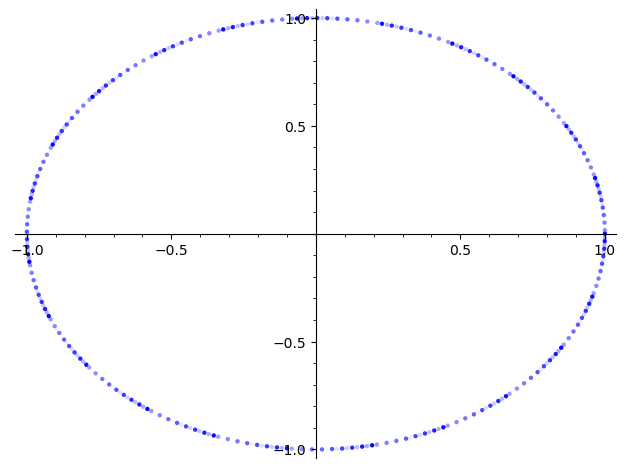
\includegraphics[width=0.5\textwidth]{graphics/irrationalRotationFig}
\end{figure}

\begin{example}\label{irrationalRotation}
One ergodic system is known as the \dfn{irrational rotation}.
Let $\theta \in [0, 2\pi]$ and suppose that $\theta/2\pi$ is irrational.
Then the map $f(z) = e^{i\theta}z$ on the circle $\Torus$, which rotates the circle by $\theta$, defines an ergodic system $(\Torus, \mu, f)$, where $\mu$ is Lebesgue measure.
The reader who is familiar with some Fourier analysis may show this in Exercise~\ref{irrational rotation exercise}.
See Figure~\ref{irrationalRotationFig}. We will study irrational rotations further in Section~\ref{nonmeasurable sets}.
\end{example}

\begin{subsec}
As a sample of the power of ergodic theory, let us prove the following theorem that ``breaks the laws of thermodynamics''.
If $(X, f)$ is a measure-preserving system and $x \in X$, we let $f^{n}(x)$ denote $f \circ \cdots \circ f$, where there are $n$ copies of $f$.
The theorem is due to Carathéodory, which is naturally why it is named after Poincar\'e.
\end{subsec}

\begin{theorem}[Poincar\'e recurrence]
Let $(X, \Sigma, P, f)$ be a measure-preserving system.
For every $A \in \Sigma$, define $A^{\flat} = \{x \in A: \forall n~f^{n}(x) \notin A\}$.
Then $P(A^{\flat}) = 0$.
\end{theorem}
\begin{proof}
We first note that
\[A^{\flat} = A \setminus \bigcup_{n \in \NN} f^{n}(A)\]
which is measurable since each of the $f^{n}(A)$ are.

If $m > n$, then $f^{n}(A^{\flat}) \cap f^{m}(A^{\flat})$ is empty: if $x \in f^{m}(A^{\flat})$, so that $f^{-m}(x) \in A^{\flat}$, then by definition of $A^{\flat}$,
\[f^{-n}(x) = f^{m-n}(f^{-m}(x)) \notin A.\]

Therefore, for any $N \in \NN$,
\[P(A^{\flat}) = \frac{1}{N} \sum_{n=1}^{N} P(f^{m}(A^{\flat})) = \frac{1}{N} P\left(\bigcup_{n=1}^{N} f^{m}(A^{\flat})\right) \leq \frac{1}{N} P(X) = \frac{1}{N}.\]
So $P(A^{\flat}) = 0$.
\end{proof}

\begin{subsec}
Let us explain to the reader who is familiar with thermodynamics how to interpret this theorem.

Let $X$ be the set of microstates that the universe can be in and let us assume for simplicity that $X$ is finite.
Let $P$ be the normalized counting measure, so that
\[P(A) = \frac{\card A}{\card X}\]
and $\Sigma = 2^{X}$.
Thus $P(A)$ represents the probability of drawing a partiular microstate uniformly at random.

Let $f: X \to X$ be the map that sends the state of the universe right now to the state of the universe one second into the future.
We can think of sets $A$ as macrostates, where $x \in A$ iff $x$ is consistent with $A$.
By Poincar\'e recurrence, if the universe is currently in macrostate $A$, then there is an $N$ such that $N$ seconds into the future, the universe will again be in macrostate $A$.
In particular, the entropy of the universe will return to what it currently is, apparently contradicting the second law of thermodynamics.
This is no contradiction, however, because $N$ is much larger than the lifespan of the universe.
\end{subsec}

\begin{subsec}
We will not discuss ergodic systems much, but ergodic theory is a crucial application of measure theory.
For example, it can be used to prove the strong law of large numbers from probability, and actually very powerful generalizations thereof.
We refer the reader to Coud\'ene~\cite{coudène2016ergodic} to learn about ergodic theory.
\end{subsec}

\begin{exercise}
Show that Poincar\'e recurrence fails for infinite measure spaces by giving a counterexample.
\end{exercise}

\begin{exercise}\label{irrational rotation exercise}
Show that the irrational rotation with Lebesgue measure forms an ergodic system.
(Hint: Let $A$ be a subset of the circle which the irrational rotation sends into itself. Consider the Fourier series of $1_{A}$. You are allowed to assume basic facts about Fourier series.)
\end{exercise}

\section{Nonmeasurable sets and infinite games}\label{nonmeasurable sets}
A $\sigma$-algebra has very strong closure properties: one needs to use some kind of operation that involves working with uncountably many sets at once to escape it.
As a consequence, every subset of $\RR$ that we have encountered is at least Lebesgue measurable, and we have not even managed to complete the proof that there is a subset of $\RR$ which is not Borel (Theorem~\ref{Borel sigma algebra}).
Lebesgue certainly hoped, but was unable to prove, that every subset of $\RR$ is Lebesgue measurable.
However, Vitali showed that this is false. In this section we will first prove Vitali's theorem, and then prove that there is a Lebesgue measurable set that is not Borel.
Since we will need some nontrivial facts from set theory, this section is optional and not used anywhere.

\begin{subsec}
We first observe that to show that there is a subset of $\RR$ which is not measurable, it suffices to do so with $\RR$ replaced by $\Torus$.
Indeed, the map $F(\theta) = e^{i\theta}$ is a measure-preserving isomorphism $F: [0, 2\pi) \to \Torus$, so if $A \subseteq \Torus$ is nonmeasurable, then $F^{-1}(A)$ is nonmeasurable as well.
\end{subsec}

\begin{subsec}
Let us recall some algebra.
If $G$ is a group and $X$ is a set, an action of $G$ on $X$ is a rule by which every $g \in G$ induces a bijection $T_g: X \to X$ which is functorial in the sense that if $h \in G$, then $T_{gh} = T_gT_h$.
Equivalently, an action of $G$ on $X$ is a morphism of groups $G \to X!$ where $X!$ is the group of all bijections $X \to X$.
If $x \in X$, the set $\{T_g(x): g \in G\}$ is known as the \dfn{orbit} of $x$.
Then we get a surjective map
\begin{align*}
S_x: G &\to \{T_g(x): g \in G\}\\
g &\mapsto T_g(x).
\end{align*}
If every such map $S_x$ is a bijection, then we say that the action is a \dfn{free action}.
\end{subsec}

\begin{subsec}
Now recall the irrational rotation, Example~\ref{irrationalRotation}.
If $\theta \in [0, 2\pi]$ is an angle and $\theta/2\pi$ is irrational, then we obtain a measure-preserving system $T: \Torus \to \Torus$, known as an irrational rotation, which acts by rotating $\Torus$ by $\theta$.
If $n \in \ZZ$, then $T^n$ acts by rotating $\Torus$ by $n\theta$.
That is, we get a group action of $\ZZ$ on $\Torus$ where $n \in \ZZ$ rotates $\Torus$ by $n\theta$.
\end{subsec}

\begin{lemma}
Every irrational rotation $\ZZ \to \Torus!$ is a free measure-preserving action.
\end{lemma}
\begin{proof}
Clearly the irrational rotation is measure-preserving, since it is a rotation and Lebesgue measure on $\Torus$ is rotation-invariant.
So we just need to show that it is free.
If not, there is $x \in \Torus$ and $q_1, q_2 \in \ZZ$ such that $T^{q_1}(x) = T^{q_2}(x)$.
Setting $q = q_2 - q_1$ we conclude $T^q(x) = x$.
In other words,
$$x + q\theta \equiv x \mod 2\pi.$$
Thus there is $N \in \ZZ$ such that $q\theta = 2\pi N$, or in other words $\theta/2\pi = N/q \in \QQ$, even though $\theta/2\pi$ is irrational.
\end{proof}

\begin{theorem}[Vitali]\label{Vitali's set}
There is a subset of $\Torus$ which is not measurable.
\end{theorem}
\begin{proof}
Choose an irrational rotation $\ZZ \to \Torus!$, let $\mathcal O$ be the set of all orbits thereof, and let $\mu$ be Lebesgue measure on $\Torus$.
Since the irrational rotation is free and $\ZZ$ is countably infinite, every element of $\mathcal O$ must also be countably infinite.
Since $\Torus$ is uncountable, $\mathcal O$ must be uncountable.
The axiom of choice, Axiom~\ref{axiom of choice}, implies that there is a set $X \subset \Torus$ which contains exactly one element from each orbit in $\mathcal O$.
Suppose that $X$ is measurable. Then $\bigcup_{q \in \ZZ} X + q = \Torus$ and the union is disjoint, so
\[1 = \mu(\Torus) = \sum_{q \in \ZZ} \mu(X + q\theta) = \sum_{q \in \ZZ} \mu(X),\]
since the irrational rotation is measure-preserving, so $\mu(X) > 0$ (so that it sums to $1$) yet $\mu(X) = 0$ (since the sum of infinitely many copies of any nonzero number is infinite and hence $> 1$), a contradiction.
\end{proof}

\begin{subsec}
Though the existence of Vitali's set may feel paradoxical, and somewhat hurts the effectiveness of $\RR^3$ as a model of ``space", it is rarely worth worrying oneself over.
Owing to the use of the axiom of choice, it is essentially impossible that a nonlogician will encounter something like Vitali's set in practice.
In fact, we will see (see the remarks at~\ref{all functions are measurable}) that virtually all sets which appear in mainstream analysis, algebra, or number theory are measurable.

On the other hand, Vitali's set shows that in logic, where the axiom of choice (and its friends such as the axiom of power set and the axiom schema of replacement) is of import, nonmeasurable sets may emerge.
But there exist models of set theory due to Solovay~\cite{Solovay1970} with certain axioms weakened where Vitali's construction fails and every subset of $\RR$ is measurable, and someone with a more constructivist bent may conclude from that theorem that indeed every set is measurable in ``reality'' (whatever that means).
Strichartz~\cite[Chapter 1]{strichartz2003guide} summarized these observations by remarking that ``wise-guys who like using the axiom of choice will have to worry about \dots wolves under the bed, etc.''
\end{subsec}

\begin{subsec}
Now let us begin the proof of Theorem~\ref{Borel sigma algebra}.
To do this, we need the notion of ``Borel complexity."
The reader should review the notion of an ordinal (see Definition~\ref{ordinal dfn}) before reading this proof.
\end{subsec}

\begin{definition}
Let $\Sigma_{1} = \mathcal T$ be the topology of $\RR$.
Given $\Sigma_{\alpha}$, $\alpha$ a countable ordinal, let $\Pi_{\alpha}$ be the set of all complements of elements of $\Sigma_{\alpha}$.
Let $\Sigma_{\alpha+1}$ be the set of countable unions of elements of $\Pi_{\alpha}$.
If $\beta < \omega_{1}$ is not equal to $\alpha+1$ for any $\alpha$, let $\Sigma_{\beta} = \bigcup_{\alpha < \beta} \Sigma_{\alpha}$.

If $A \subseteq \RR$ is a Borel set and $\Sigma_{\alpha}$ or $\Pi_{\alpha}$ is the smallest set in the above construction such that $A \in \Sigma_{\alpha}$ or $A \in \Pi_{\alpha}$, we say that $A$ has \dfn{Borel complexity} $\Sigma_{\alpha}$ or $\Pi_{\alpha}$.
The set $\{\Sigma_{\alpha}, \Pi_{\alpha}\}_{\alpha}$ of all Borel complexity classes is called the \dfn{Borel hierarchy}.
\end{definition}

\begin{subsec}
By transfinite recursion (Theorem~\ref{transfinite induction}), for every countable ordinal $\alpha$, $\Sigma_{\alpha}$ and $\Pi_{\alpha}$ are well-defined.
Every open set has Borel complexity $\Sigma_{1}$ and every closed set has Borel complexity $\Pi_{1}$.
\end{subsec}

\begin{subsec}
Here is a diagram of the first few stages of the Borel hierarchy:
$$\begin{tikzcd}
\Pi_{1} \arrow[drdr,dashed,blue] && \Pi_{2} \arrow[drdr,dashed,blue] && \Pi_{3} \arrow[drdr,dashed,blue] && \cdots\\\\
\Sigma_{1} \arrow[urur,dotted,red] && \Sigma_{2} \arrow[urur,dotted,red] && \Sigma_{3} \arrow[urur,dotted,red] && \cdots
\end{tikzcd}$$
The dashed blue arrows indicate taking countable intersections, while the dotted red arrows indicate taking countable unions.
At every stage, $\Pi_{\alpha}$ consists of the complements of elements of $\Sigma_{\alpha}$.
\end{subsec}

\begin{lemma}
Every Borel set has a well-defined Borel complexity.
\end{lemma}
\begin{proof}
The set $A$ was obtained by applying countable union and complement countably many times to an open set, and thus is in $\Sigma_{\omega_{1}} = \bigcup_{\alpha < \omega_{1}} \Sigma_{\alpha}$.
\end{proof}

\begin{subsec}
One may wonder if there are sets of Borel complexity $\Sigma_{\alpha}$ for every countable ordinal $\alpha$. In fact, there are; see \cite[Corollary 2.38]{Marker2002}.
\end{subsec}

\begin{subsec}
Recall (Definition~\ref{beth dfn}) that $\beth_{1}$ is the cardinality of $\RR$, which is well-defined by Theorem~\ref{well-ordering theorem}; meanwhile $\beth_{2}$ is the cardinality of the set of all subsets of $\RR$.
\end{subsec}

\begin{lemma}
If $\alpha$ is a countable ordinal, then
$$\card \Sigma_{\alpha} = \card \Pi_{\alpha} = \beth_{1}.$$
\end{lemma}
\begin{proof}
We proceed by transfinite induction.
By Theorem~\ref{cardinality of topology}, $\Sigma_{0}$ has cardinality $\beth_{1}$.
The mapping $A \mapsto A^{c}$ is a bijection $\Sigma_{\alpha} \to \Pi_{\alpha}$.

If $\Pi_{\alpha}$ has cardinality $\beth_{1}$ then so does $\Sigma_{\alpha+1}$, since each element of $\Sigma_{\alpha+1}$ can be expressed in terms of a countable number of elements of $\Pi_{\alpha}$, and $\beth_{1} \times \beth_{1} \times \cdots$ has cardinality $\beth_{1}$ by Theorem~\ref{cardinal arithmetic trivial}.

Finally if $\beta$ is a countable limit ordinal and for every $\alpha < \beta$, $\Sigma_{\alpha}$ is countable, then $\Sigma_{\beta}$ is a countable union of sets of cardinality $\beth_{1}$, hence has cardinality $\beth_{1}$ by Theorem~\ref{cardinal arithmetic trivial}.
It follows by induction that for every countable ordinal $\alpha$, $\Sigma_{\alpha}$ has cardinality $\beth_{1}$.
\end{proof}

\begin{theorem}[Theorem~\ref{Borel sigma algebra}, redux]\label{Borel not Lebesgue}
The Borel $\sigma$-algebra of $\RR$ has cardinality $\beth_{1}$, which is strictly less than the cardinality $\beth_{2}$ of the Lebesgue $\sigma$-algebra.
In particular, there is a Lebesgue measurable set which is not Borel.
\end{theorem}
\begin{proof}
Let $\Sigma$ be the Borel $\sigma$-algebra. Then
$$\Sigma = \bigcup_{\alpha} \Sigma_{\alpha}.$$
The set of all countable ordinals has cardinality $\aleph_{1}$, and $\aleph_{1} \leq \beth_{1}$ (by Theorem~\ref{well-ordering theorem} and the fact that $\beth_{1}$ is uncountable).
So
$$\card \Sigma = \aleph_{1} \cdot \beth_{1} = \beth_{1}$$
by Theorem~\ref{cardinal arithmetic trivial}.

On the other hand, the Lebesgue $\sigma$-algebra contains every null set, and in particular contains every subset of a null Cantor set.
A Cantor set has cardinality $\beth_{1}$, so its power set has cardinality $\beth_{2}$.
By Cantor's diagonal argument, $\beth_{1} < \beth_{2}$.
Since there are more Lebesgue measurable sets than Borel sets, there must a Lebesgue measurable set which is not Borel.
\end{proof}

\begin{subsec}
Lebesgue falsely claimed~\cite{Lebesgue1905} that the continuous image of a Borel set is Borel.
In fact, Souslin~\cite{Souslin1917} showed that there exists a \dfn{projective set} -- a set which can be obtained from Borel sets by taking continuous images and complements finitely many times -- which is not Borel.
For a discussion of the history of Lebesgue's blunder see MathOverflow~\cite{MO34142}.
\end{subsec}

\begin{subsec}
One may reasonably ask if every projective set is Lebesgue measurable.
To discuss this, we need the notion of a \dfn{Gale-Stewart game}, which is just a set $A \subseteq [0, 1]$.
The set defines a game in which the players, Alice and Bob, take turns choosing digits; Alice picks first.
After countably many rounds, the players have given a real number $x \in [0, 1]$.
Alice wins iff $x \in A$, and otherwise Bob wins.
\end{subsec}

\begin{definition}
Let $A \subseteq [0, 1]$ be a Gale-Stewart game. Then:
\begin{enumerate}
\item We say that \dfn{Alice has a winning strategy} for $A$ if there is a digit $x_1$ which Alice can pick such that no matter what digit $x_2$ Bob picks, Alice can pick a digit $x_3$ such that no matter what digit $x_4$ Bob picks, and so on, Alice will win in the sense that $0.x_1x_2x_3x_4\dots \in A$.
\item We say that \dfn{Bob has a winning strategy} for $A$ if for every digit $x_1$ that Alice picks, there is a digit $x_2$ that Bob can pick such that no matter what digit $x_3$ that Alice picks, there is a digit $x_4$ that Bob can pick, and so on, Bob will win in the sense that $0.x_1x_2x_3x_4\dots \notin A$.
\item If either Alice or Bob have a winning strategy, we say that $A$ is a \dfn{determined game}.
\end{enumerate}
\end{definition}

\begin{theorem}[Martin-Steel projective determinancy theorem~\cite{SteelMartin10.2307/1990913}]
Every projective set is determined.
\end{theorem}

\begin{subsec}
Every determined game is Lebesgue measurable; see Exercise~\ref{determined games are measurable}.
So, if we believe the projective determinacy theorem, every projective set is measurable.
However, there is just one catch: Martin and Steel needed to use axioms for set theory much stronger than the usual axioms for set theory discussed in Section~\ref{axioms of set theory} to prove their theorem, and this is optimal in the sense that a weaker set of axioms for set theory cannot prove the projective determinacy theorem.
\end{subsec}

\begin{exercise}
Let $A \subseteq \RR$ be a measurable set.
Show that either $A$ is null, or $A$ has a nonmeasurable subset.
\end{exercise}

\begin{exercise}[\cite{pugh2013real}]
Show that the continuous (or even smooth, if you are brave) image of a Lebesgue measurable set may not be measurable.
(Hint: Let $C$ be a null Cantor set and $F$ be a ``fat" Cantor set, so $F$ has positive Lebesgue measure.
Send a null subset $C$ to a nonmeasurable subset of $F$.)
\end{exercise}

\begin{exercise}
Show that for every Lebesgue measurable set $E \subseteq \RR$ there is a set $F$ of complexity $\Pi_2$ and a set $D$ of complexity $\Sigma_2$ such that
$$D \subseteq E \subseteq F$$
and $F \setminus D$ is null. (Hint: Lebesgue measure is a Radon measure.)
\end{exercise}

\begin{exercise}[Gale-Stewart]
Prove that every open subset of $[0, 1]$ is determined.
\end{exercise}

\begin{exercise}\label{determined games are measurable}
Assume that $A$ is a determined game such that every measurable subset of $A$ is null.
Show that $A$ is null, and therefore measurable.
Conclude that every determined game is measurable, and in particular that Vitali's set is not determined.
\end{exercise}

\begin{exercise}[Zermelo]
The game of chess consists of two players, White and Black.
White is more likely to win than Black if both players are equally skilled.
So consider chess, modified so that if there is a draw, then Black automatically wins.
Assume that there is $N$ such that every game of chess is at most $N$ turns long (this is a nice exercise in recreational mathematics if one knows the rules of chess), and at every turn, White and Black have at most $N$ valid moves.
Show that chess can be viewed as a Gale-Stewart game $A$, and that $A$ is determined.
\end{exercise}
